\section{Runge-Kutta-Verfahren}

\vspace{1\baselineskip}

Geg.: $\dot{\vec{y}} = \vec{f}(t,\vec{y})$ wobei $\vec{y} (t_0) = \vec{y}_0$

Ges.: Lösung $\vec{y}(t)$ des AWP 1. Ordnung

Idee: Schreibe das DGLproblem in ein Integrationsproblem um:
$\vec{y}(t_1) = \vec{y}(t_0) + \int_{t_0}^{t_1} \vec{f}(t,\vec{t}) dt$ und verwende eine
Quadraturformel zur Approximation des Integrals:

$\vec{y} (t_1) \approx \vec{y}_0 + h \sum_{i=1}^s b_i \vec{f}(t_0 + c_i h , \vec{y} (t_0 + c_i h))$

mit Gewichten $b_i$ und Stützstellen $c_i \in [0,1]$ und $h=t_1-t_0$

\pagebreak

\fat{Explizite Mittelpunktsregel}

Wir wählen die Mittelpunktsregel als QF. Der noch unbekannte Funktionswert in der
Mitte $y(t_0 + \frac{h}{2})$ wird durch eE approximiert.

\begin{center}
    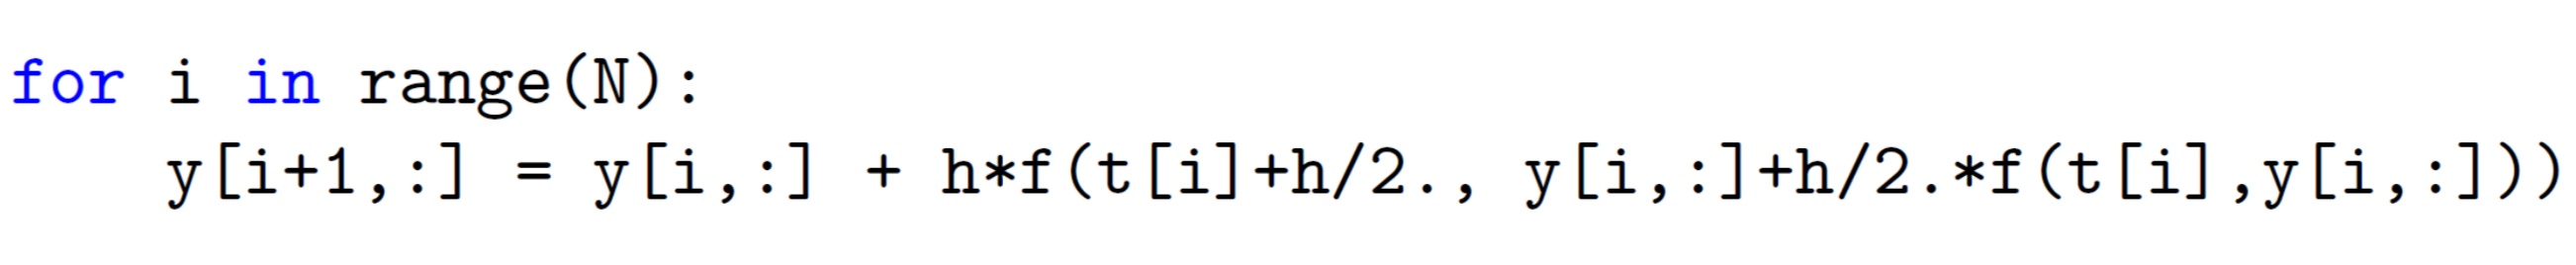
\includegraphics[width=0.45\textwidth]{Figures/RK_eM.png}
\end{center}

Mit der Notation für allgemeine RK Verfahren lässt sich dies schreiben als:
$\vec{k}_1 := \vec{f}(t_0,\vec{y}(t_0))$ und
$\vec{k}_2 := \vec{f}(t_0 + \frac{h}{2} , \vec{y}_0 + \frac{h}{2} \vec{k}_1)$.
Dann ist $\vec{y}_1 = \vec{y}_0 + h \vec{k}_2$.

\vspace{1\baselineskip}

\fat{Explizite Trapezregel}

Wir wählen die Trapezregel als QF. Der noch unbekannte Funktionswert $y(t_0 + h)$ wird
durch eE approximiert.

\begin{center}
    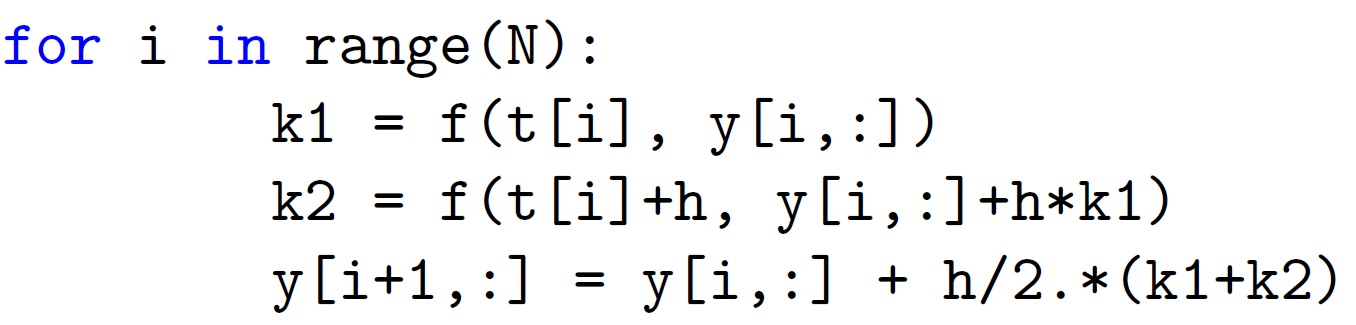
\includegraphics[width=0.25\textwidth]{Figures/RK_eT.png}
\end{center}

$\vec{k}_1 := \vec{f}(t_0 , \vec{y} (t_0))$ und
$\vec{k}_2 := \vec{f}(t_0 + h , \vec{y}(t_0) + h \vec{f}(t_0, \vec{y}_0))$,
dann ist $\vec{y}_1 = \vec{y}_0 + \frac{h}{2} (\vec{k}_1 + \vec{k}_2)$

\vspace{1\baselineskip}

\fat{Polygonzugverfahren}: Die drei Polygonzugverfahren sind jeweils $s=1$-stufige RK
Verfahren.

\vspace{1\baselineskip}

\fat{s-stufiges RK-Verfahren}

Gegeben sind $b_i$ und $a_{ij}$ in $\R$ mit $i,j = 1,\dots,s$ und $\sum_{i=1}^s b_i = 1$.
Dann ist $c_i := \sum_{j=1}^s a_{ij}$ und definiere:

\vspace{1\baselineskip}

\fat{Vorgehen}: (Allgemeines RK-Verfahren)

Berechne: $\vec{k}_i := \vec{f}(t_0 + c_i h , \vec{y}_0 + h \sum_{j=1}^s a_{ij} \vec{k}_j)$
\ \ mit $i=1,\dots,s$

Daraus: $\vec{y}_{j+1} = \vec{y}_j + h \sum:{i=1}^s b_i \vec{k}_i$

\vspace{1\baselineskip}

\Definition{

    Das \fat{Butcher-Tableau} zur Darstellung eines RK-Verfahrens:

    \begin{center}
        \begin{tabular}{c|ccc}
            $c_{1}$ & $a_{11}$ & $\dots$ & $a_{1 s}$ \\
            $\vdots$ & $\vdots$ & & $\vdots$ \\
            $c_{s}$ & $a_{s 1}$ & $\dots$ & $a_{s s}$ \\
            \hline & $b_{1}$ & $\dots$ & $b_{s}$
            \end{tabular} \ \ $=:$ \ \ \begin{tabular}{c|c}
            $\vec{c}$ & $A$ \\
            \hline
            & $(\vec{b})^T$
        \end{tabular}
    \end{center}    
}

Ein RK-Verfahren heisst:
\begin{itemize}
    \item \fat{explizit}, falls $A$ eine strikte untere Dreiecksmatrix ist. Da sich jedes
        $k_i$ aus den früher berechneten $k_i$'s bestimmen lässt, müssen keine inpliziten
        Gleichungen gelöst werden.
    \item \fat{diagonal implizit}, falls $A$ eine nicht-strikte untere Dreiecksmatrix ist.
        Es kann nacheinander eine Gleichung für das neue $k_i$ aufgestellt werden.
    \item \fat{implizit}, sonst. Es muss eine grosse Gleichung mit allen $k_i$'s als
        Unbekannten auf eine Schlange gelöst werden. Dies benötigt den grössten und
        kompliziertesten Rechenaufwand.
\end{itemize}

\vspace{1\baselineskip}

\fat{Beispiele}:

\vspace{1\baselineskip}

eE:
\begin{tabular}{c|c}
    $0$ & $0$ \\
    \hline & $1$
\end{tabular}
\quad
iE: \begin{tabular}{c|c}
    $1$ & $1$ \\
    \hline & $1$
\end{tabular}
\quad
iM: \begin{tabular}{c|c}
    $\frac{1}{2}$ & $\frac{1}{2}$ \\
    \hline & $1$
\end{tabular}

\vspace{1\baselineskip}

eT: \begin{tabular}{c|cc}
    $0$ & $0$ & $0$ \\
    $1$ & $1$ & $0$ \\
    \hline & $\frac{1}{2}$ & $\frac{1}{2}$ 
\end{tabular}
\quad
eM: \begin{tabular}{c|cc}
    $0$ & $0$ & $0$ \\
    $\frac{1}{2}$ & $\frac{1}{2}$ & 0 \\
    \hline & $0$ & $1$
\end{tabular}

\pagebreak

\underline{\fat{Gauss-Kollokation}}

\underline{Motivation}: Nutze Analog zu Gauss-Legendre QF die maximale Ordnung eines
$s$-stufigen RK-Verfahrens aus:
\begin{itemize}
    \item Explizites Verfahren: Ordnung $p \leq s$
    \item Implizites Verfahren: Ordnung $p \leq 2s$
\end{itemize}
\underline{Idee}: Approximiere $y(t)$ zwischen $t_0$ und $t_0 + h$ durch ein
Polynom von Grad $s$ (= Kollokationspolynom $u(t)$), welches die DGL an den Punkten
$t_0 + c_i h \in [t_0 , t_0 + h]$ erfüllt:
\begin{align*}
    \begin{cases}
        u(t_0) = y_0 \\
        \dot{u}(t + c_i h) = f(t_0 + c_i h , u(t_0+c_i h)) \ \
        \forall i \in \geschwungeneklammer{1,\dots,s}
    \end{cases}
\end{align*}
Lösen mit: RK-Verfahren mit $a_{ij} := \int_0^{c_i} l_j (t) dt$,
$b_i := \int_0^1 l_i (t) dt$ mit $l_i(t)$ den Lagrange-Polynomen $\forall i \in
\geschwungeneklammer{1,\dots,n}$ und $c_i$ den Knoten der Gauss-Legendre-QF
(hier: Knoten $\hat{=}$ NST des $s$-ten verschobenen Legendre Polynomes
$P_s (x) := \frac{ds}{dx^s} (x^s (x-1)^s)$)

\vspace{1\baselineskip}

\underline{Konkret}:
Kollokationsverfahren sind implizite RK-Verfahren mit speziellen Einträgen im
Butcher-Tableau.

\vspace{1\baselineskip}

\Beispiel{ (Gauss-Koll. zu $s=2$)

\vspace{1\baselineskip}

    \begin{tabular}{c|cc}
        $\frac{1}{2} - \frac{\sqrt{3}}{6}$ & $\frac{1}{4}$ & $\frac{1}{2} - \frac{\sqrt{3}}{6}$ \\
        $\frac{1}{2} + \frac{\sqrt{3}}{6}$ & $\frac{1}{4} + \frac{\sqrt{3}}{6}$ & $\frac{1}{4}$ \\
        \hline & $\frac{1}{2}$ & $\frac{1}{2}$
    \end{tabular}

    Knoten $c_{1,2} = \frac{1}{2} \pm \frac{\sqrt{3}}{6}$
}

\vspace{1\baselineskip}

\underline{\fat{Adaptivität/ Partitioniertes RK}}

Bisher: Schrittweite $h$= konst.

\underline{Idee}: Verkleinere $h$, wo $f$ schwierig, vergrössere $h$ wo $f$ einfach.

\underline{Vorgehen}: Verwende zwei RK-Verfahren unterschiedlicher Ordnung
(Code: $\Psi_{\text{high}}$, $\Psi_{\text{low}}$) und berechne den lokalen Fehler.
$\Rightarrow$
\begin{itemize}
    \item lok. Fehler gross: $h_{\text{neu}} := \frac{h}{2}$
    \item lok. Fehler klein: $h_{\text{neu}} := c \cdot h$ ($c > 1)$ zB. $1.1$
\end{itemize}

\underline{Wichtig!}: rhs mus formell Zeitabhängig sein!
